% WebContactsProPlus — layered architecture
\documentclass[border=14pt]{standalone}
\usepackage{tikz}
\usetikzlibrary{positioning, arrows.meta, shapes.geometric, fit, calc, backgrounds}

\begin{document}
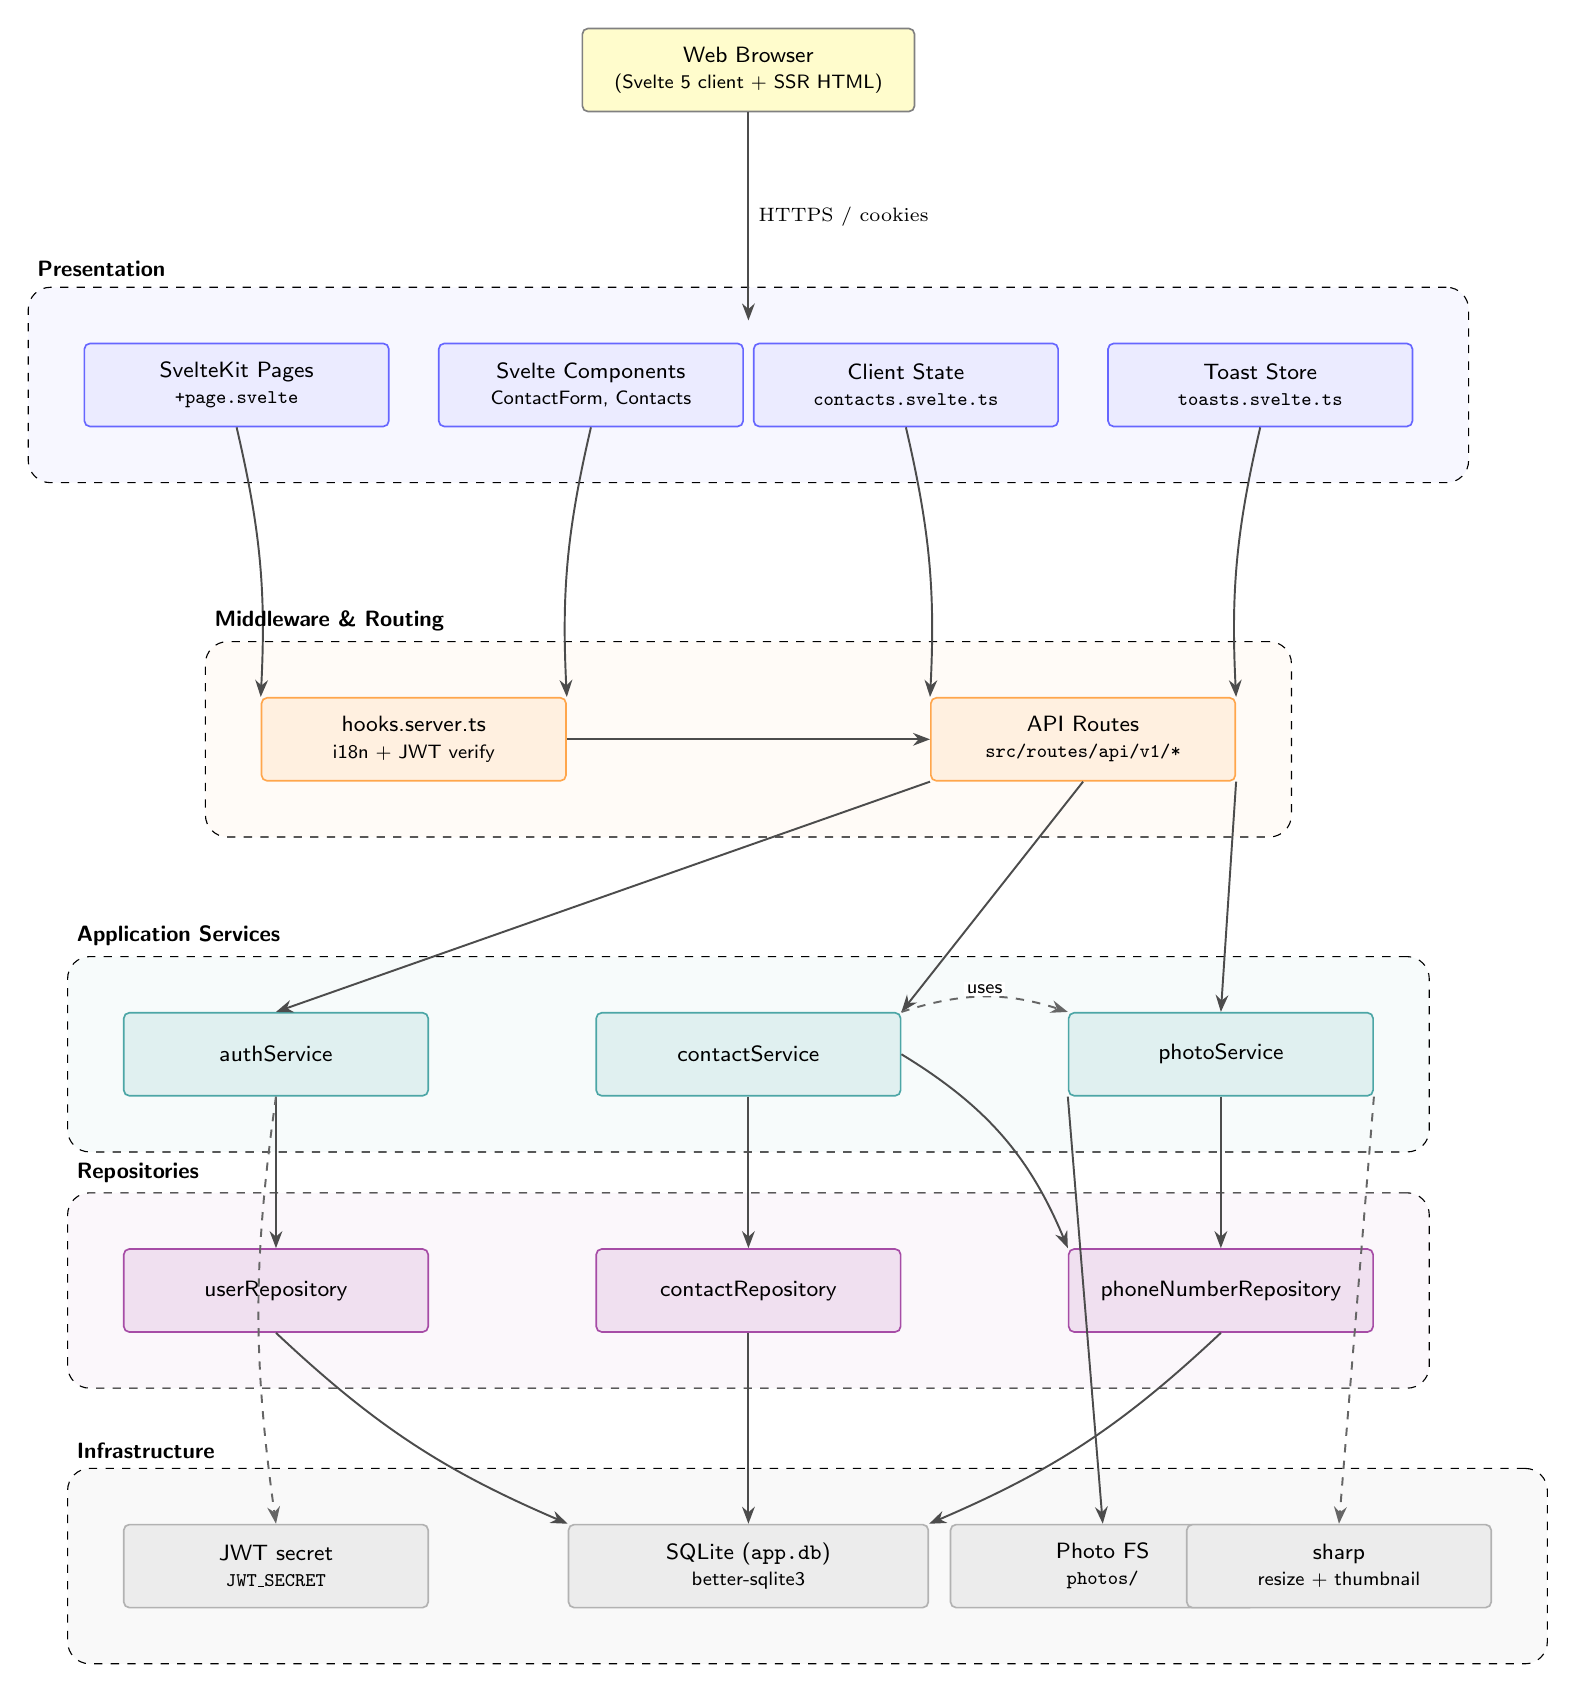
\begin{tikzpicture}[
    >=Stealth,
    font=\sffamily\small,
    box/.style={
        draw, rounded corners=2pt, line width=0.6pt,
        minimum height=30pt, minimum width=110pt,
        align=center, font=\sffamily\footnotesize,
        fill=white,
    },
    layer/.style={draw, dashed, rounded corners=8pt, inner sep=20pt},
    presentation/.style={box, fill=blue!8,   draw=blue!60},
    middleware/.style={box,   fill=orange!12, draw=orange!70},
    service/.style={box,      fill=teal!12,   draw=teal!70},
    repo/.style={box,         fill=violet!12, draw=violet!70},
    infra/.style={box,        fill=gray!15,   draw=gray!60},
    actor/.style={box,        fill=yellow!20, draw=black!50, minimum width=120pt},
    arrow/.style={->, line width=0.7pt, draw=black!70},
    darrow/.style={->, line width=0.7pt, draw=black!60, dashed},
    layertitle/.style={font=\sffamily\bfseries\footnotesize, anchor=west},
    bigbus/.style={line width=0.7pt, draw=black!70},
]

% ============ NODES ============

% Browser
\node[actor] (browser) at (8, 2.5) {Web Browser \\ {\scriptsize (Svelte 5 client + SSR HTML)}};

% Presentation row (y=-1.5)
\node[presentation] (pages)      at (1.5,  -1.5) {SvelteKit Pages \\ {\scriptsize \texttt{+page.svelte}}};
\node[presentation] (components) at (6,    -1.5) {Svelte Components \\ {\scriptsize ContactForm, Contacts}};
\node[presentation] (state)      at (10,   -1.5) {Client State \\ {\scriptsize \texttt{contacts.svelte.ts}}};
\node[presentation] (toasts)     at (14.5, -1.5) {Toast Store \\ {\scriptsize \texttt{toasts.svelte.ts}}};

% Middleware row (y=-6) — hooks centered under Pages/Components, routes under State/Toasts
\node[middleware] (hooks)  at (3.75,  -6) {hooks.server.ts \\ {\scriptsize i18n + JWT verify}};
\node[middleware] (routes) at (12.25, -6) {API Routes \\ {\scriptsize \texttt{src/routes/api/v1/*}}};

% Services row (y=-10)
\node[service] (authsvc)    at (2,   -10) {authService};
\node[service] (contactsvc) at (8,   -10) {contactService};
\node[service] (photosvc)   at (14,  -10) {photoService};

% Repositories row (y=-13)
\node[repo] (userrepo)    at (2,   -13) {userRepository};
\node[repo] (contactrepo) at (8,   -13) {contactRepository};
\node[repo] (phonerepo)   at (14,  -13) {phoneNumberRepository};

% Infrastructure row (y=-16.5) — column-aligned with consumers
\node[infra, minimum width=110pt] (jwt)     at (2,    -16.5) {JWT secret \\ {\scriptsize \texttt{JWT\_SECRET}}};
\node[infra, minimum width=130pt] (sqlite)  at (8,    -16.5) {SQLite (\texttt{app.db}) \\ {\scriptsize better-sqlite3}};
\node[infra, minimum width=110pt] (photofs) at (12.5, -16.5) {Photo FS \\ {\scriptsize \texttt{photos/}}};
\node[infra, minimum width=110pt] (sharp)   at (15.5, -16.5) {sharp \\ {\scriptsize resize + thumbnail}};

% ============ ARROWS ============

% Browser → Presentation (one arrow into the layer at its top center)
\draw[arrow] (browser.south) --
    node[right, font=\scriptsize]{HTTPS / cookies}
    ($(components.north)!0.5!(state.north)+(0,8pt)$);

% Presentation → Middleware: each box drops to its nearest target
\draw[arrow] (pages.south)      to[bend left=8]  (hooks.north west);
\draw[arrow] (components.south) to[bend right=8] (hooks.north east);
\draw[arrow] (state.south)      to[bend left=8]  (routes.north west);
\draw[arrow] (toasts.south)     to[bend right=8] (routes.north east);

% hooks ↔ routes (within middleware)
\draw[arrow] (hooks.east) -- (routes.west);

% Middleware → Services: routes fans out to all three services (straight diagonals are clean — no boxes in between)
\draw[arrow] (routes.south west) -- (authsvc.north);
\draw[arrow] (routes.south)      -- (contactsvc.north east);
\draw[arrow] (routes.south east) -- (photosvc.north);

% Services → Repositories (vertical, column-aligned)
\draw[arrow] (authsvc.south)    -- (userrepo.north);
\draw[arrow] (contactsvc.south) -- (contactrepo.north);
\draw[arrow] (photosvc.south)   -- (phonerepo.north);

% Cross-arrow: contactService also uses phoneNumberRepository — route AROUND contactRepository on the right
\draw[arrow] (contactsvc.east) to[bend left=18] (phonerepo.north west);

% Cross-arrow: contactService → photoService (cascade delete) — bend ABOVE the services row
\draw[darrow] (contactsvc.north east) to[bend left=18]
    node[above, font=\sffamily\scriptsize, fill=white, inner sep=1pt]{uses}
    (photosvc.north west);

% Repositories → SQLite (three converging, entry points spread on sqlite.north)
\draw[arrow]  (userrepo.south)    to[bend right=10] (sqlite.north west);
\draw[arrow]  (contactrepo.south) -- (sqlite.north);
\draw[arrow]  (phonerepo.south)   to[bend left=10]  (sqlite.north east);

% Services / repos → other Infrastructure (column-aligned, vertical)
\draw[darrow] (authsvc.south)        to[bend right=8] (jwt.north);
\draw[arrow]  (photosvc.south west)  -- (photofs.north);
\draw[darrow] (photosvc.south east)  -- (sharp.north);

% ============ LAYER BACKGROUNDS + TITLES ============
\begin{pgfonlayer}{background}
    \node[layer, fill=blue!3,   fit=(pages)(components)(state)(toasts)] (pl) {};
    \node[layer, fill=orange!3, fit=(hooks)(routes)]                    (ml) {};
    \node[layer, fill=teal!3,   fit=(authsvc)(contactsvc)(photosvc)]    (sl) {};
    \node[layer, fill=violet!3, fit=(userrepo)(contactrepo)(phonerepo)] (rl) {};
    \node[layer, fill=gray!5,   fit=(sqlite)(photofs)(sharp)(jwt)]      (il) {};
\end{pgfonlayer}

\node[layertitle, anchor=south west] at (pl.north west) {Presentation};
\node[layertitle, anchor=south west] at (ml.north west) {Middleware \& Routing};
\node[layertitle, anchor=south west] at (sl.north west) {Application Services};
\node[layertitle, anchor=south west] at (rl.north west) {Repositories};
\node[layertitle, anchor=south west] at (il.north west) {Infrastructure};

\end{tikzpicture}
\end{document}
